\documentclass[12pt]{TA-Rifky-Matematika}
\usepackage{graphicx}
\usepackage{booktabs}
\usepackage{amsmath,amssymb}
\usepackage{longtable}
\usepackage{float}
\usepackage{tikz}
\renewcommand{\tablename}{Tabel}
\renewcommand{\figurename}{Gambar}

% IDENTITAS TUGAS AKHIR -- ubah nilai di bawah ini
\JudulTA{JUDUL TUGAS AKHIR DALAM BAHASA INDONESIA}
\Title{Thesis Title in English}
\NamaMahasiswa{Nama Lengkap Mahasiswa}
\NamaKapital{NAMA LENGKAP MAHASISWA}
\NIMMahasiswa{12XXXXXXXX}
\ProgramStudi{Matematika}
\NamaFakultas{Sains}
\TahunTA{2026}

% DOSEN DAN PENGESAHAN
\PB1{Dr. Rifky Fauzi, S.Si., M.Si.}
\NIPPB1{NIP 199203242022031006}
\PB2{Nama Pembimbing 2}
\NIPPB2{NIP 199XXXXXXXXXXXXX}
\PB3{}
\NIPPB3{}
\KoorProdi{Nama Koor Prodi}
\NIPKoorProdi{NIP 19XXXXXXXXXXXXXX}
\TanggalPengesahan{5 November 2026}

\begin{document}
\nomenclature{$x$}{Variabel atau besaran yang didefinisikan dalam penelitian}

\MulaiBagianDepan
\HalamanSampul
\HalamanPengesahan{Gambar/placeholder-foto.png}
\PernyataanOrisinalitas
\PersetujuanPublikasi
\begin{Abstrak}
Tuliskan abstrak yang memuat masalah penelitian, tujuan, metode, hasil utama, dan kesimpulan secara ringkas. Ganti paragraf ini dengan ringkasan penelitian yang telah selesai.

\textbf{Kata kunci:} kata kunci pertama; kata kunci kedua; kata kunci ketiga.

\end{Abstrak}
\begin{Abstract}
Write the abstract describing the research problem, objective, methods, principal results, and conclusion. Replace this paragraph with the final research abstract.

\textbf{Keywords:} first keyword; second keyword; third keyword.

\end{Abstract}
\HalamanKataPengantar
Puji syukur penulis panjatkan kepada Tuhan Yang Maha Esa atas terselesaikannya tugas akhir ini. Penulis menyampaikan terima kasih kepada para pembimbing dan pihak yang mendukung penyusunan naskah. Uraian ini perlu disesuaikan dengan kondisi sebenarnya.

\begin{flushright}
Lampung Selatan, 5 November 2026\\[2ex]
Penulis
\end{flushright}

% Hapus dua bagian di bawah ini bila tidak digunakan.
\HalamanPersembahanTA
Halaman persembahan bersifat opsional. Ganti kalimat ini dengan isi persembahan atau hapus kedua baris pemanggil halaman ini pada \texttt{main.tex}.

\HalamanMottoTA
Halaman motto bersifat opsional. Ganti kalimat ini dengan motto pribadi atau hapus kedua baris pemanggil halaman ini pada \texttt{main.tex}.

\CetakDaftarIsi
\CetakDaftarGambar
\CetakDaftarTabel
\CetakDaftarSimbol

\MulaiIsiTA
\chapter{PENDAHULUAN}
\section{Latar Belakang}
Uraikan konteks masalah, kesenjangan penelitian, dan alasan ilmiah penelitian perlu dilakukan. Dukungan literatur yang relevan wajib disitasi dengan perintah \texttt{\textbackslash cite} menggunakan kunci pustaka pada berkas \texttt{Referensi.bib}.
\section{Rumusan Masalah}
Nyatakan pertanyaan penelitian yang spesifik, terukur, dan dapat dijawab melalui metode yang dipilih.
\section{Tujuan Penelitian}
Nyatakan tujuan yang berkorespondensi langsung dengan rumusan masalah.
\section{Manfaat Penelitian}
Jelaskan kontribusi teoretis atau penerapan yang diharapkan.
\section{Batasan Masalah}
Tegaskan ruang lingkup, asumsi, dan keterbatasan penelitian.

\chapter{TINJAUAN PUSTAKA}
\section{Penelitian Terdahulu}
Sintesis penelitian relevan dan jelaskan posisi penelitian yang dilakukan, bukan hanya rangkuman artikel.
\section{Landasan Teori}
Definisikan istilah, konsep, dan hasil matematika yang benar-benar digunakan.
\begin{definition}
Misalkan $x\in\mathbb{R}$. Definisi ini merupakan contoh lingkungan pernyataan matematis yang perlu diganti sesuai topik penelitian.
\end{definition}
Contoh persamaan bernomor:
\begin{equation}\label{eq:contoh}
 f(x)=x^2.
\end{equation}
Persamaan~\eqref{eq:contoh} hanya merupakan contoh penulisan.

\chapter{METODOLOGI PENELITIAN}
\section{Jenis dan Rancangan Penelitian}
Jelaskan rancangan penelitian beserta alasan pemilihan pendekatan.
\section{Data, Sumber, atau Asumsi Model}
Uraikan objek, data, parameter, asumsi, serta cara memperoleh atau membangunnya.
\section{Tahapan Penelitian}
Jelaskan urutan pekerjaan sehingga setiap tahapan memiliki keluaran yang dapat diperiksa.
\section{Metode Analisis dan Validasi}
Jelaskan metode yang menjawab setiap rumusan masalah, termasuk pengujian, verifikasi, atau validasi sesuai bidang penelitian.

\chapter{HASIL DAN PEMBAHASAN}
\section{Contoh Penyajian Gambar}
Gambar~\ref{fig:kurva} memperlihatkan contoh kurva $y=x^2$ yang dibuat sendiri menggunakan \texttt{TikZ}. Gambar ini merupakan ilustrasi mandiri, bukan reproduksi dari publikasi lain. Apabila gambar diadaptasi dari sumber luar, sumber aslinya wajib disebutkan dalam keterangan gambar dan daftar pustaka.
\begin{figure}[htbp]
\centering
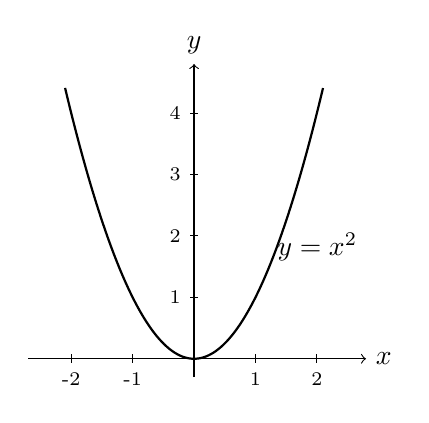
\begin{tikzpicture}[scale=0.78]
  \draw[->] (-2.7,0) -- (2.8,0) node[right] {$x$};
  \draw[->] (0,-0.3) -- (0,4.8) node[above] {$y$};
  \draw[thick,domain=-2.1:2.1,samples=100,smooth] plot (\x,{\x*\x});
  \node[above right] at (1.2,1.44) {$y=x^2$};
  \foreach \x in {-2,-1,1,2} {\draw (\x,0.07)--(\x,-0.07) node[below] {\scriptsize \x};}
  \foreach \y in {1,2,3,4} {\draw (0.06,\y)--(-0.06,\y) node[left] {\scriptsize \y};}
\end{tikzpicture}
\caption{Ilustrasi kurva fungsi kuadrat (sumber: dibuat oleh penulis)}
\label{fig:kurva}
\end{figure}

\section{Contoh Penyajian Tabel dan Rujukan}
Tabel~\ref{tab:contoh} memuat nilai fungsi yang diperoleh secara analitik. Data pada tabel merupakan contoh perhitungan, bukan hasil penelitian. Pembahasan metode perhitungan dan kestabilan numerik dapat merujuk pada sumber akademik yang relevan, misalnya \cite{higham2002}.
\begin{table}[htbp]
\centering
\caption{Nilai fungsi $f(x)=x^2$ pada beberapa titik (sumber: perhitungan penulis)}
\label{tab:contoh}
\begin{tabular}{cc}
\toprule
$x$ & $f(x)$ \\
\midrule
0 & 0 \\
1 & 1 \\
2 & 4 \\
\bottomrule
\end{tabular}
\end{table}

\section{Pembahasan}
Jelaskan makna temuan, hubungan dengan teori, perbandingan dengan literatur, serta batasan yang relevan. Pastikan setiap gambar dan tabel dirujuk dari teks; jangan hanya menampilkannya tanpa analisis.

\chapter{KESIMPULAN DAN SARAN}
\section{Kesimpulan}
Tuliskan jawaban ringkas terhadap setiap rumusan masalah, berdasarkan hasil yang telah disajikan.
\section{Saran}
Sampaikan pengembangan lanjutan yang secara langsung timbul dari keterbatasan dan temuan penelitian.

\CetakReferensi{Referensi}
\MulaiLampiranTA{DOKUMEN PENDUKUNG}
Tempatkan data tambahan, bukti perhitungan, algoritma, atau dokumen pendukung yang perlu dilampirkan.

\end{document}
